%%%%%%%%%%%%%%%%%%%%%%%%%%%%%%%%%%%%%%%%%%%%%%%%%%%%%%%%%%%%%%%%%%%%%%%%%%%%%%%%
%2345678901234567890123456789012345678901234567890123456789012345678901234567890
%        1         2         3         4         5         6         7         8

\documentclass[letterpaper, 10 pt, conference]{ieeeconf}  % Comment this line out
                                                          % if you need a4paper
%\documentclass[a4paper, 10pt, conference]{ieeeconf}      % Use this line for a4
                                                          % paper

\IEEEoverridecommandlockouts                              % This command is only
                                                          % needed if you want to
                                                          % use the \thanks command
\overrideIEEEmargins
% See the \addtolength command later in the file to balance the column lengths
% on the last page of the document



% The following packages can be found on http:\\www.ctan.org
%\usepackage{graphics} % for pdf, bitmapped graphics files
%\usepackage{epsfig} % for postscript graphics files
%\usepackage{mathptmx} % assumes new font selection scheme installed
%\usepackage{times} % assumes new font selection scheme installed
%\usepackage{amsmath} % assumes amsmath package installed
%\usepackage{amssymb}  % assumes amsmath package installed
\usepackage{graphicx}
\title{\LARGE \bf
Instruction-level Parallelism in Computing Contour Trees
}

%\author{ \parbox{3 in}{\centering Huibert Kwakernaak*
%         \thanks{*Use the $\backslash$thanks command to put information here}\\
%         Faculty of Electrical Engineering, Mathematics and Computer Science\\
%         University of Twente\\
%         7500 AE Enschede, The Netherlands\\
%         {\tt\small h.kwakernaak@autsubmit.com}}
%         \hspace*{ 0.5 in}
%         \parbox{3 in}{ \centering Pradeep Misra**
%         \thanks{**The footnote marks may be inserted manually}\\
%        Department of Electrical Engineering \\
%         Wright State University\\
%         Dayton, OH 45435, USA\\
%         {\tt\small pmisra@cs.wright.edu}}
%}

\author{Mattin Mir-Tahmasebi (Username: mm5213, CID: 00824754)}


\begin{document}



\maketitle
\thispagestyle{empty}
\pagestyle{empty}





%%%%%%%%%%%%%%%%%%%%%%%%%%%%%%%%%%%%%%%%%%%%%%%%%%%%%%%%%%%%%%%%%%%%%%%%%%%%%%%%
\section{Varying RUU Size}

The approach began by determining the best register update unit (RUU) size by measuring the instructions per cycle (IPC) and the total energy consumed for different values. As is seen in Figure \ref{fig:energy_ruu}, the lowest energy consumption occurs at an RUU size of 16. This can be explained by looking at Figure \ref{fig:ipc_ruu}, which shows that the marginal throughput diminishes after an RUU of size 16. So, increasing RUU size from 2 to 16 decreased power usage, because the energy saved from using fewer cycles outweighed the increased energy from a larger RUU, but after size 16 this benefit is not seen, because the larger RUU is drawing more energy but not providing extra throughput in return, so power usage rises again.

\begin{figure}[h]
	\begin{center}
	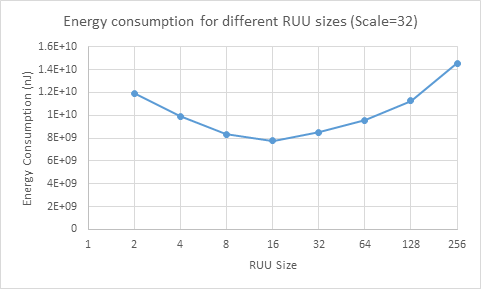
\includegraphics[width=0.4\textwidth]{Energy_RUU.png}\\
  	\caption{Energy consumption for different RUU sizes}
    \label{fig:energy_ruu}
    \end{center}
\end{figure}

\begin{figure}[h]
	\begin{center}
	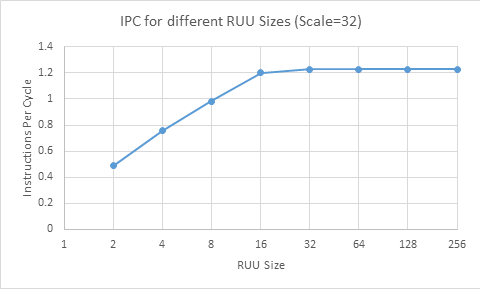
\includegraphics[width=0.4\textwidth]{IPC_RUU.png}\\
  	\caption{Instructions Per Cycle for different RUU sizes}
    \label{fig:ipc_ruu}
    \end{center}
\end{figure}

\section{Branch Predictor}
The next parameter to be varied was the branch predictor. For a general purpose machine, having a naive branch predictor (taken/nottaken) would not be optimal, but since our problem domain is specific, it is possible for a more naive, less power-consuming approach to be best. 

Figure \ref{fig:bpred} shows that the naive predictors were much worse than the perfect predictor, with around 1.5x the energy usage, as opposed to the more advanced predictors which used around 1.3x the energy. Note that the naive predictors had a much worse comparative cycle count than they did comparative energy usage - we can attribute this to the simpler predictors requiring less energy to function, so even though they are incorrect more often, causing the cycle count to increase, their reduced energy usage outweighs this to a degree.

\begin{figure}[h]
	\begin{center}
	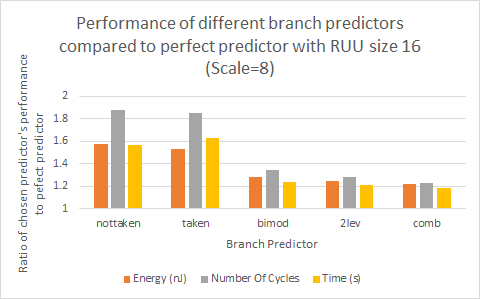
\includegraphics[width=0.4\textwidth]{bpred.png}\\
  	\caption{Branch Predictors as Compared to a Perfect Predictor}
    \label{fig:bpred}
    \end{center}
\end{figure}

\end{document}
